%------------------------------------------------

\begin{fullwidth}
Many research questions require the team to acquire original data,
because no source of publicly available data addresses the
inputs or outcomes of interest for the relevant population.
Data acquisition can take many forms, including:
primary data generated through surveys;
private sector partnerships granting access to new data sources, such as administrative and sensor data;
digitization of paper records, including administrative data; web scraping;
primary data capture by unmanned aerial vehicles or other types of remote sensing;
or novel integration of various types of datasets, such as combining survey and sensor data.
Much of the recent push toward credibility in the social sciences has focused on analytical practices.
However, credible development research depends, first and foremost, on the quality of the acquired data.
Clear and careful documentation of the data acquisition process is essential for research reproducibility.

This chapter covers reproducible data acquisition,
special considerations for generating high-quality survey data,
and protocols for safely and securely handling confidential data.
The first section discusses reproducible data acquisition:
how to establish and document your right to use the data.
This applies to all original data,
whether collected for the first time through surveys or sensors or acquired through a unique partnership.
The second section goes into detail on data acquisition through surveys,
as this process is typically more involved than acquisition of secondary data,
and has more in-built opportunities for quality control.
It provides detailed guidance on the electronic survey workflow,
from designing electronic survey instruments to monitoring data quality once fieldwork is ongoing.
The final section discusses safe data handling,
providing guidance on how to receive, transfer, store, and share confidential data.
Secure file management is a basic requirement to comply with the legal and
ethical agreements that allow  access to personal information for research purposes.


\end{fullwidth}

\section{Acquiring data ethically}

Clearly establishing and documenting data access is critical for reproducible research.
This section provides guidelines for 
establishing data ownership, receiving data from development partners,
and documenting the research team's right to use the data.
It is the researchers' responsibility to respect the rights
of people who own the data and the people who are described by it;
but also to make sure that information is as available and accessible as possible.
These twin responsibilities can and do come into tension,
so it is important to be fully informed about what other researchers are doing
and to fully inform other researchers of what you are doing.
Writing down and agreeing to specific details is a good way of doing that.


\subsection{Data ownership}
Before acquiring any data, it is critical to establish data ownership.
Data ownership\sidenote{\url{https://dimewiki.worldbank.org/Data_Ownership}}\index{data ownership}
can sometimes be challenging to establish,
as various jurisdictions have differing laws regarding data and information,
and the research team may have their own information regulations.
In some, data is implicitly owned by the people who it is about.
In others, it is owned by the people who collected it.
In still more, it is highly unclear and there are varying norms.
The best approach is always to consult with a local partner,
and enter into specific legal agreements establishing ownership,
access, and publication rights.
This is particularly critical where confidential data is involved
-- that is, when people are disclosing information to you
that you could not obtain simply by observation or through public records.

If the research team is requesting access to existing data, 
they must enter into data licensing agreements\index{data licensing}
to access the data and publish research outputs based on it.
These agreements should make clear from the outset whether the
research team can make the original data, any portion thereof, or derivatives\sidenote{
	\textbf{Derivatives} of data can be indicators, aggregates,
	visualizations etc. created from the original data.}
of the data, public.
If the data is publicly accessible, 
this may be as simple to agreeing to terms of use on the website where the data can be downloaded. 
If it is original data that is not yet publicly accessible, 
the process is typically more complex and requires a documented legal agreement or memorandum of understanding.

If the research team is generating data directly, such as survey data,
it is important to clarify up front who owns the data,
and who will have access to it.
These details need to be shared with respondents when they are offered the opportunity
to consent to participate in the study.
If the research team is not collecting the data directly --
for example, if a government, private company, or research partner is doing the data collection --
make sure that you have an explicit agreement
about who owns the resulting data.

The contract for data collection should include specific terms
as to the rights and responsibilities of each stakeholder.
It must clearly stipulate which party owns the data produced,
and that the research team maintains full intellectual property rights.
The contract should also explicitly indicate that the contracted firm
is responsible for protecting respondent privacy,
that the data collection will not be delegated to any third parties,
and that the data will not be used by the firm or subcontractors for any purpose not expressly stated in the contract,
before, during or after the assignment.
The contract should also stipulate that the vendor is required to comply with
ethical standards for social science research,
and adhere to the specific terms of agreement with the relevant
Institutional Review Board (IRB)\sidenote{
	\url{https://dimewiki.worldbank.org/IRB\_Approval}}
or applicable local authority.
Finally, it should include policies on reuse, storage, and retention or destruction of data.

Research teams that acquire original data must also consider data ownership downstream,
through the terms they will use to release that data to other researchers or to the general public.
The team should consider whether they can publish the data in full after removing personal identifiers.
For example, the team must consider whether it would be acceptable for
their data to be copied and stored on servers anywhere in the world,
whether they would prefer to manage permissions on a case-by-case basis,
and whether they expect that data users would cite or credit them.
Similarly, the team can require users in turn to release
their derivative datasets or publications under similar licenses,
or offer use without restriction.
There are simple license templates for offering many of these permissions,
but, at the planning stage, the team should make sure
that all licensing agreements, data collection contracts,
and informed consent processes
used to acquire the data specifically detail those future uses.


\subsection{Data licensing}

Data licensing\sidenote{
	\url{https://dimewiki.worldbank.org/Data_License_Agreement}}
is the formal act of the dataset owner
giving some data rights to a specific user,
while retaining ownership of the dataset.
If you are not the owner of the dataset you want to analyze,
you must enter into a licensing agreement to access it for research purposes.
Similarly, when you own a dataset,
you must consider whether you will make the dataset accessible to other researchers,
and what terms-of-use you require.

If the research team requires access to existing data for novel research,
terms of use should be agreed on with the data owner,
typically through a data licensing agreement.
These terms should specify what data elements will be received,
what purpose the data will be used for, and who will have access to the data.
Keep in mind that the data owner is likely not highly familiar
with the research process, and therefore may be surprised
at some of the things you want to do if you are not clear up front.
You will typically want intellectual property rights to all research outputs developed used the data,
a license for all uses of derivative works, including public distribution
(unless ethical considerations contraindicate this).
This is important to allow the research team to store, catalog, and publish, in whole or in part,
either the original licensed dataset or datasets derived from the original.
Make sure that the license you obtain from the data owner allows these uses,
and that you consult with the owner
if you foresee exceptions with specific portions of the data.

The World Bank has a template Data License Agreement which DIME follows.
The template specifies the specific objectives of the data sharing,
and whether the data can be used only for the established purpose
or for other objectives after it is obtained.
It classifies the data into one of four access categories,
depending on who can access the data by default
and whether case-by-case authorization for access is needed.
The data provider may impose similar restrictions
to sharing derivative data and any or all of the associated metadata.
The template also specifies the required citation for the data.
While you do not need to use the World Bank's template
or its access categories if you do not work on a World Bank project,
we still think it is important that you use this information in two ways.
First, make sure to base your Data License Agreement on some template.
Hand-written agreements can leave many legal ambiguities or gaps
where the permissions given to the research team are unclear or incomplete.
Second, we strongly recommend you to categorize data using some variation of this system.
Then you should have different standard procedures for each category,
so that the intended processes for handling the data are clear.


\subsection{Receiving data from development partners}

Research teams granted access to existing data may receive that data in a number of different ways.
You may receive access to an existing server,
or physical access to extract certain information,
or a one-time data transfer.
In all cases, you must take action to ensure
that data is transferred through
secure channels so that confidentiality is not compromised.
See the section \textit{Handling data securely} later in this chapter for how to do that.
Keep in mind that compliance with ethical research standards may
in some cases require a stricter level of security than initially proposed by the partner agency.
It is also critical at this stage to request any and all available documentation for the data;
this could take the form of a data dictionary, codebook, 
manual for administrative data collection system, reports,
among others. 
If no written documentation is available, 
interview the person(s) responsible for managing the data,
to learn as much as possible about the data; 
the interview notes should be archived with data documentation.

At this stage, it is very important to assess
documentation and cataloging of the data and associated metadata.
It is not always clear what pieces of information will jointly constitute a research dataset,
and many of the datasets you receive will not be organized for research.
You should always retain the original data exactly as received
alongside a copy of the corresponding ownership agreement or license.
You should make a simple \texttt{README} document noting the date of receipt,\index{README}
the source and recipient of the data,
and a brief description of each file received.
All too often data will be provided as vaguely-named spreadsheets,
or digital files with non-specific titles,
and documentation will be critical for future access and reproducibility.

Eventually, you will want to make sure that you are creating a set of documents
that can be properly submitted to a data catalog and given a reference and citation.
The metadata -- documentation about the data -- is critical for future use of the data.
Metadata should include documentation of how the data was created,
what they measure, and how they are to be used.
In the case of survey data, this includes the survey instrument and associated manuals;
the sampling protocols and field adherence to those protocols, and any sampling weights;
what variable(s) uniquely identify the dataset(s), and how different datasets can be linked;
and a description of field procedures and quality controls.
DIME uses as a standard the Data Documentation Initiative (DDI), which is supported by the
World Bank's Microdata Catalog.\sidenote{\url{https://microdata.worldbank.org}}

As soon as the desired pieces of information are stored together,
think about which ones are the components of what you would call a dataset.
Often, when you are receiving data from a partner,
even highly-structured materials such as registers or records
are not, as received, equivalent to a research dataset,
and require initial cleaning, restructuring, or recombination
to reach the stage we would consider a raw research dataset.
This is as much an art than a science:
you want to keep information together that is best contextualized together,
but you also want to information granular as much as possible,
particularly when there are varying units of observation.
There usually won't be a single correct way to answer this question,
and the research team will need to decide how the materials received.
Soon, you will begin to build research datasets from this set of information,
and these will become your original clean data,
which will be the material published, released, and cited
as the starting point of your data.
(If funders or publishers request that ``raw'' data be published or cataloged,
for example, this is the dataset that you should provide.)
These first datasets created from the received materials
are the objects you need to catalog, release, and license.
Now is a good time to being assessing disclosure risk
and/or seek publication licenses in collaboration with data providers,
while you are in close contact with them.



%------------------------------------------------


\section{Collecting high-quality data using electronic surveys}
In this section, we detail specific considerations
for acquiring high-quality data through electronic surveys of study subjects.
There are many excellent resources on questionnaire design and field supervision,
but few that cover the particular challenges and opportunities presented by electronic surveys.
There are also many survey software options available to researchers,
and the market is rapidly evolving.
Therefore, we focus on specific workflow considerations for digitally-collected data,
and on basic concepts rather than software-specific tools.

Electronic data collection technologies
have greatly accelerated our ability to bring in high-quality data
using purpose-built survey instruments,
and therefore improved the precision of research.
At the same time, electronic surveys create new pitfalls to avoid.
Programming electronic surveys efficiently requires a very different mindset 
than writing paper-based surveys;
careful preparation can improve survey efficiency and data quality.
This section will outline the major steps and technical considerations
you will need to follow whenever you field a custom survey instrument,
no matter the scale.

\subsection{Designing survey instruments}
A well-designed questionnaire results from careful planning,
consideration of analysis and indicators,
close review of existing questionnaires,
survey pilots, and research team and stakeholder review.\sidenote{
	\url{https://dimewiki.worldbank.org/Questionnaire\_Design}}
There are many excellent resources on questionnaire design,
such as from the World Bank's Living Standards Measurement Survey.\sidenote{\citet{glewwe2000designing}}
The focus of this section is the design of electronic field surveys,
often referred to as Computer Assisted Personal Interviews (CAPI).\sidenote{
  \url{https://dimewiki.worldbank.org/Computer-Assisted\_Personal\_Interviews\_(CAPI)}}
Although most surveys are now collected electronically, by tablet, mobile phone or web browser,
\textbf{questionnaire design}
  \index{questionnaire design}
(content development) and \textbf{questionnaire programming}\sidenote{
  \url{https://dimewiki.worldbank.org/Questionnaire\_Programming}}
(functionality development) should be seen as two strictly separate tasks.
Therefore, the research team should agree on all questionnaire content
and design a version of the survey on paper
before beginning to program the electronic version.
This facilitates a focus on content during the design process
and ensures teams have a readable, printable version of their questionnaire.
Most importantly, it means the research, not the technology,
drives the questionnaire design.

We recommend this approach for three reasons.
First, an easy-to-read paper questionnaire
is very useful for training data collection staff, 
which we will discuss further in the enumerator training section below.
Second, finalizing the paper version of the questionnaire before beginning any programming
avoids version control concerns that arise from concurrent work
on paper and electronic survey instruments.
Third, a readable paper questionnaire is a necessary component of data documentation,
since it is difficult to work backwards from the survey program to the intended concepts.

The workflow for designing a questionnaire will feel much like writing an essay:
begin from broad concepts and slowly flesh out the specifics.\sidenote{
  \url{https://dimewiki.worldbank.org/Questionnaire_Design}}\index{questionnaire design}
It is essential to start with a clear understanding of the
\textbf{theory of change}\sidenote{
  \url{https://dimewiki.worldbank.org/Theory\_of\_Change}}\index{theory of change}
and \textbf{research design}\sidenote{
  \url{https://dimewiki.worldbank.org/Research\_Design}}\index{research design}
  for your project.
The first step of questionnaire design is to list key outcomes of interest,
as well as the main covariates to control for and any variables needed for the specific research design.
The ideal starting point for this is a \textbf{pre-analysis plan}.\sidenote{
  \url{https://dimewiki.worldbank.org/Pre-Analysis\_Plan}}\index{pre-analysis plan}

Use the list of key outcomes to create an outline of questionnaire \textit{modules}.
Do not number the modules; instead use a short prefix
as numbers quickly get outdated when modules are reordered.
For each module, determine if the module is applicable to the full sample,
or only to specific respondents,
and whether or how often the module should be repeated.
A few examples:
a module on maternal health only applies
to households with a woman who has children,
a household income module should be answered
by the person responsible for household finances,
and a module on agricultural production
might be repeated for each crop the household cultivated.
Each module should then be expanded
into specific indicators to observe in the field.\sidenote{
  \url{https://dimewiki.worldbank.org/Literature\_Review\_for\_Questionnaire}}
Questionnaires for impact evaluation
must also include ways to document the reasons for \textbf{attrition} and
treatment \textbf{contamination}.\index{attrition}\index{contamination}
These are essential data components for completing CONSORT records,
a standardized system for reporting enrollment, intervention allocation, follow-up,
and data analysis through the phases of a randomized trial.\sidenote{\citet{begg1996improving}}

\subsection{Piloting survey instruments}
A \textbf{survey pilot}\sidenote{
 \url{https://dimewiki.worldbank.org/Piloting\_Survey\_Content}}\index{survey pilot}
is a critical to finalize survey design.\sidenote{
	\url{https://dimewiki.worldbank.org/Survey\_Pilot}}
The pilot must be done out-of-sample,
but in a context as similar as possible to the study sample.
The survey pilot includes three steps:
a \textbf{pre-pilot}, a \textbf{content-focused pilot}, and a \textbf{data-focused pilot}.\sidenote{
	\url{https://dimewiki.worldbank.org/Structuring\_a\_Survey\_Pilot}}
The first step is a \textbf{pre-pilot}.
The pre-pilot is a qualitative exercise, done early in the questionnaire design process.
The objective is to answer broad questions about how to measure key outcome variables,
and gather qualitative information relevant to any of the planned survey modules.
A pre-pilot is particularly important when designing new survey instruments.

The second step is a \textbf{content-focused pilot}\sidenote{
  \url{https://dimewiki.worldbank.org/Piloting\_Survey\_Content}}.
The objectives at this stage are to improve the structure and length of the questionnaire,
refine the phrasing and translation of specific questions,
check for potential sensitivities” and for enumerator/respondent interactions,
and confirm coded response options are exhaustive.\sidenote{
	\url{https://dimewiki.worldbank.org/index.php?title=Checklist:\_Refine\_the\_Questionnaire\_(Content)}}
In addition, it is an opportunity to test and refine all survey protocols,\sidenote{
	\url{https://dimewiki.worldbank.org/Piloting\_Survey_Protocols}}
such as how units will be sampled or pre-selected units identified.
The content-focused pilot is best done on pen and paper, before the questionnaire is programmed,
because changes at this point may be deep and structural,
which are hard to adjust in code.
It is important at this point to test both the validity and the reliability 
of the survey questions; 
for this reason it is important to conduct the content-focused pilot
with a sufficiently large sample (the exact requirement will depend on the research sample;
a very rough rule of thumb is a minimum of 30 interviews.

After testing the content, proceed to program a draft version
of the electronic survey instrument.
The final stage is a \textbf{data-focused pilot}.
The objective at this stage is to refine the questionnaire programming;
this is discussed in more detail in the following section.\sidenote{
	\url{https://dimewiki.worldbank.org/Timeline\_of\_Survey\_Pilot}}


\subsection{Programming electronic survey instruments}
Once the team is satisfied with the content and structure of the survey,
it is time to move on to implementing it electronically.
Electronic data collection has great potential
to simplify survey implementation and improve data quality.
But it is critical to ensure that electronic survey instruments 
flow correctly and produce data that can be used in statistical software, 
before data collection starts.
Electronic questionnaires are typically developed
in a spreadsheet (usually using Excel or Google Sheets)
or a software-specific form builder,
all of which are accessible even to novice users.\sidenote{
  \url{https://dimewiki.worldbank.org/Questionnaire\_Programming}}
We will not address software-specific form design in this book;
rather, we focus on coding and design conventions that are important to follow
for electronic surveys regardless of software choice.\sidenote{
  \url{https://dimewiki.worldbank.org/SurveyCTO\_Coding\_Practices}}
Survey software tools provide a wide range of features
designed to make implementing even highly complex surveys
easy, scalable, and secure.
However, these are not fully automatic:
you need to actively design and manage the survey.
Here, we discuss specific practices that you need to follow
to take advantage of electronic survey features
and ensure that the exported data
is compatible with your statistical software.

From a data perspective, questions with \textbf{coded response options}\sidenote{
  \textbf{Coded response options:} Responses to questions which require respondents
  to select from a list of choices, corresponding to underlying numerical response codes.}\index{coded response options}
are always preferable to \textbf{open-ended questions}.\sidenote{
  \textbf{Open-ended questions:} Responses to questions which do not
  impose any structure on the response, typically recorded as free-flowing text.}\index{open-ended questions}
The content-based pilot is an excellent time to ask open-ended questions
and refine fixed responses for the final version of the questionnaire --
do not count on coding up lots of free text after a full survey.
Coding responses helps to ensure that the data
will be useful for quantitative analysis.
Two examples help illustrate the point.
First, instead of asking ``How do you feel about the proposed policy change?'',
use techniques like \textbf{Likert scales}.\sidenote{
  \textbf{Likert scale:} an ordered selection of choices indicating the respondent's level of agreement or disagreement with a proposed statement.}
Second, if collecting data on things like medication use or food supplies, you could collect:
the brand name of the product; the generic name of the product; a coded identifier for the item;
or the broad category to which each product belongs
(``antibiotics'' or ``staple foods'', for example).\sidenote{
  See \citet{wafula2017examining} for an example.}
All four may be useful for different reasons,
but the latter two are likely to be the most useful for rapid data analysis.
The coded identifiers require providing a translation dictionary to field staff,
but enables automated rapid recoding for analysis with no loss of information.
The broad category requires agreement on the groups of interest,
but allows for much more comprehensible top-line statistics and data quality checks.
Rigorous field testing is required to ensure that answer categories are comprehensive;
however, it is best practice to include an \textit{other, specify} option.
Keep track of those responses in the first few weeks of field work.
Adding an answer category for a response frequently showing up as \textit{other} can save time,
as it avoids extensive post-coding.

It is essential to name the fields in your questionnaire
in a way that will also work in your data analysis software.
Most survey programs will not enforce this by default,
since limits vary across statistical software,
and survey software will encourage you
to use long sentences as question labels
and detailed descriptions as choice options.
This is what you want for the enumerator-respondent interaction,
but you should already have analysis-compatible labels programmed in the background
so the resulting data can be rapidly imported in analytical software.
There is some debate over how exactly individual questions should be identified:
formats like \texttt{hq\_1} are hard to remember and unpleasant to reorder,
but formats like \texttt{hq\_asked\_about\_loans} quickly become cumbersome.
We recommend using descriptive names with clear prefixes so that variables
within a module stay together when sorted alphabetically.\sidenote{
  \url{https://dimewiki.worldbank.org/Variable_Names}}\index{variable naming}
Variable names should never include spaces or mixed cases
(we prefer all-lowercase naming).
Take special care with the length: very long names will be cut off in some softwares,
which could result in a loss of uniqueness and lots of manual work to restore compatibility.
We further discourage explicit question numbering,
at least at first, as it discourages re-ordering questions,
which is a common recommended change after the pilot.
In the case of follow-up surveys, numbering can quickly become convoluted,
too often resulting in uninformative variables names like
\texttt{ag\_15a}, \texttt{ag\_15\_new}, \texttt{ag\_15\_fup2}, and so on.

\subsection{Using electronic survey features to enhance data quality}
Electronic surveys are more than simply
a paper questionnaire displayed on a mobile device or web browser.
All common survey software allows you to automate survey logic
and include hard or soft constraints on survey responses.
These features make enumerators' work easier,
and they create the opportunity to identify and resolve
data issues in real time,
simplifying data cleaning and improving response quality.
Well-programmed questionnaires should include
most or all of the following features:

\begin{itemize}
  \item{\textbf{Localization}}: the survey instrument should display full-text questions and responses in all potential survey languages, and it should also have English and code-compatible versions of all text and labels.
	\item{\textbf{Survey logic}}: built-in tests should be included for all logic connections between questions, so that only relevant questions appear, rather than relying on enumerators to follow complex survey logic. This covers simple skip codes, as well as more complex interdependencies (e.g., a child health module is only asked to households that report the presence of a child under 5).
	\item{\textbf{Range checks}}: add range checks for all numeric variables to catch data entry mistakes (e.g. \texttt{age} must be less than 120).
	\item{\textbf{Confirmation of key variables}}: require double entry of essential information (such as a contact phone number in a survey with planned phone follow-ups), with automatic validation that the two entries match and rejection and re-entry otherwise.
	\item{\textbf{Multimedia}}: electronic questionnaires facilitate collection of images, video, and geolocation data directly during the survey, using the camera and GPS built into the tablet or phone.
	\item{\textbf{Preloaded data}}: data from previous rounds or related surveys can be used to prepopulate certain sections of the questionnaire, and validated during the survey.
	\item{\textbf{Filtered response options}}: filters reduce the number of response options dynamically (e.g. filtering a ``cities'' choice list based on the state selected).
	\item{\textbf{Location checks}}: enumerators submit their actual location using in-built GPS, to confirm they are in the right place for the interview.
	\item{\textbf{Consistency checks}}: check that answers to related questions align, and trigger a warning if not so that enumerators can probe further (e.g., if a household reports producing 800 kg of maize, but selling 900 kg of maize from their own production).
	\item{\textbf{Calculations}}: make the electronic survey instrument do all math, rather than relying on the enumerator or asking them to carry a calculator.
\end{itemize}

All established survey software include debugging and test options
to correct syntax errors and make sure that
the survey instruments will successfully compile.
This is not sufficient, however, to ensure that the resulting dataset
will load without errors in your data analysis software of choice.
DIME Analytics developed the \texttt{ietestform} command,\sidenote{
  \url{https://dimewiki.worldbank.org/ietestform}}\index{ietestform}
part of the Stata package \texttt{iefieldkit},\index{iefieldkit}
to implement a form-checking routine for \textbf{SurveyCTO},
a proprietary implementation of the open source \textbf{Open Data Kit (ODK)} software.
Intended for use during questionnaire programming and before field work,
\texttt{ietestform} tests for best practices
in coding, naming and labeling, and choice lists.
Although \texttt{ietestform} is software-specific,
many of the tests it runs are general and important to consider regardless of software choice.
To give a few examples, \texttt{ietestform} tests that no variable names exceed
32 characters, the limit in Stata (variable names that exceed that limit will
be truncated, and as a result may no longer be unique).
It checks whether ranges are included for numeric variables.
\texttt{ietestform} also removes all leading and trailing blanks from response lists,
which could be handled inconsistently across software.

The final stage of survey piloting, the data-focused pilot, should be done at this stage (after the questionnaire is programmed).
The objective of this \textbf{data-focused pilot}\sidenote{
  \url{https://dimewiki.worldbank.org/index.php?title=Checklist:\_Refine\_the\_Questionnaire\_(Data)}}
is to validate the programming and export a sample dataset.
Significant desk-testing of the instrument is required to debug the programming
as fully as possible before going to the field.
It is important to plan for multiple days of piloting,
so that any debugging or other revisions to the electronic survey instrument
can be made at the end of each day and tested the following, until no further field errors arise.
The data-focused pilot should be done in advance of enumerator training.

\subsection{Training Enumerators}
Once a survey instrument is designed, piloted on paper to refine content, 
programmed, piloted electronically to refine the data,
and fully translated to any local language(s), 
it is time to prepare to train the field staff who will be 
responsible for conducting interviews. 
The following guidelines for enumerator training apply regardless of 
whether data will ultimately be collected in person or remotely,
with the only significant differences being in terms of survey protocols and 
the nature of the field practice (which could be in-person or by phone).

The first step is to develop a detailed \textbf{enumerator manual}.\sidenote{
  For more details on how to design an enumerator manual 
  and a template for enumerator manuals
  see the DIME Wiki:
  \url{https://dimewiki.worldbank.org/wiki/Enumerator\_Training\#Enumerator\_manual}}
	\index{enumerator manual}
The manual should explain each question in the survey instrument,
address any issues that arose during piloting
and cover frequently asked questions.
The manual must also describe survey protocols and conventions,
such as how to select or confirm the identity of respondents,
and standardized means for recording responses such as ``Don't know''.\sidenote{
  For more details and examples of common survey protocols
  see the DIME Wiki:
  \url{https://dimewiki.worldbank.org/Survey\_Protocols}}
\index{survey protocols}
The enumerator manual serves as the basis for the \textbf{enumerator training}.
	\index{enumerator training}
We recommend the training to be divided into two sessions:
first a training-of-trainers, and then the enumerator training. 
The training-of-trainers should include the field supervisors and survey managers, 
and should be led by the research team.
The objective is to ensure the survey leaders are 
deeply familiar with the survey instrument and protocols,
so that they can support and supervise enumerators going forward. 
The training-of-trainers typically lasts a few days,
though exact length will depend on the complexity of the 
survey instrument and experience level of the staff. 

Enumerator training includes all field staff,
and should be jointly led by the research team 
and the survey managers.\sidenote{
  More deatails and best practices related to enumerator trainings 
  can be found on the DIME Wiki: 
  \url{https://dimewiki.worldbank.org/Enumerator\_Training}} 
This training typically lasts one to two weeks, 
though exact length will depend on complexity and experience; 
training for particularly challenging surveys may take a full month.
Enumerator training has three components: review of the paper questionnaire,
review of the electronic survey instrument, and field practice. 
The training schedule should allow for significant discussion and feedback
after each component. 
Training with a paper survey instrument is critical, 
even for surveys that will be deployed electronically. 
Starting with paper ensures a focus on survey content and structure
before diving into the technical components of the survey software.
It is much easier for enumerators to understand
the overall flow of a survey instrument and 
the range of possible participant responses
on a paper survey than on a tablet,
and it is easier to translate that understanding to 
digital functionality later.\sidenote{DIME Analytics
	developed standard guidelines for introducing field staff 
	to the survey software DIME uses most commonly, SurveyCTO: 
	\url{https://osf.io/n7ctd/}}
The classroom training should be very interactive, using methods such as role plays
and mock interviews to test understanding of survey protocols and modules.
The field practice should be carefully supervised, 
so as to provide individualized feedback to each enumerator. 
Enumerators should submit data from practice interviews to the server,
and the research team should run the standard data quality checks,
to familiarize the enumerators with that standards for data quality 
and how quality issues will be communicated and resolved. 
It is essential to train more enumerators than will be required 
for the survey, 
and to include objective assessments throughout the training.\sidenote{For a more
	detailed discussion of assessment metrics, see the DIME Wiki: 
	\url{https://dimewiki.worldbank.org/Enumerator\_Training/Assessing\_Enumerators}}
These assessments can take the form of pop quizzes (which we recommend doing daily,
using the same software as the survey), points for participation, 
and score on the field practice. 
At the end of the training, use the aggregate score to transparently select the final team of enumerators.


\subsection{Real-time data quality checks}
Once all field staff are trained, it is time to start collecting data.
If you have followed all the guidance above, the stage should be set for quality data.
To ensure high quality data in practice, 
the research team should develop a \textbf{data quality assurance plan}.\sidenote{For a
	detailed discussion of how to develop a Data Quality Assurance plan, see the DIME Wiki:
	\url{https://dimewiki.worldbank.org/Data\_Quality\_Assurance\_Plan}}
A key advantage of electronic data collection methods,
as compared to traditional paper surveys and one-time data dumps,
is the ability to access and analyze the data as data collection is ongoing.
Data issues can then be identified and resolved in real-time.
Designing systematic data checks and running them routinely throughout data collection
simplifies field monitoring and improves data quality.
There are two important types of checks for data quality monitoring: 
high frequency quality checks and field validation.\sidenote{For a comprehensive discussion
	of monitoring data quality, see the DIME Wiki: \url{https://dimewiki.worldbank.org/Monitoring\_Data\_Quality}}

\textbf{High frequency data quality checks} should be scripted 
in advance of the start of data collection,
so that data checks can start as soon as data starts to come in. 
A research assistant should run the high-frequency checks (HFCs) on a daily basis 
for the duration of the survey.\sidenote{To learn more about what types of checks should be included in the HFCs,
	see the DIME Wiki: \url{https://dimewiki.worldbank.org/High\_Frequency\_Checks}}
HFCs should include monitor consistency and range of responses to each question, 
survey programming validation, tests for enumerator-specific effects, 
and checks for duplicate entries and completeness of online submissions vis-a-vis the field log.

High-frequency checks will only improve data quality
if the issues they catch are communicated to the data provider
and corrections are documented and applied to the data.
This requires close communication with the field team, 
so that enumerators are made aware of data quality issues promptly,
and a transparent system for document issues and corrections. 
There are many ways to communicate results of high-frequency checks to the field team.
What's most important is to find a way to create actionable information for your team.
\texttt{ipacheck}, for example, generates a spreadsheet with flagged errors;
these can be sent directly to the data collection teams.
Many teams choose other formats to display results,
such as online dashboards created by custom scripts.
It is also possible to automate communication of errors to the field team
by adding scripts to link the HFCs with a messaging platform.
Any of these solutions are possible:
what works best for your team will depend on such factors as
cellular networks in field work areas, whether field supervisors have access to laptops,
internet speed, and coding skills of the team preparing the HFC workflows.

Careful \textbf{field validation} is essential for high-quality survey data.
While we cannot control natural measurement error,\sidenote{
	See \citet{kondylis2015measuring} for an example.}
which comes from variation in the realization of key outcomes,
there is often an opportunity to reduce error arising from inaccuracies in the data generation process.
\textbf{Back-checks}, spotchecks and other validation audits help ensure that 
data is not falsified, incomplete, or otherwise suspect.\sidenote{For instructions
	on how to design and implement Back Checks, see the DIME Wiki: \url{https://dimewiki.worldbank.org/Back\_Checks}}
Field validation is also an opportunity to ensure that all field protocols are followed.
For back-checks, a random subset of observations is selected,
and a subset of information from the full survey is
verified through a brief targeted survey with the original respondent.
For spot-checks, field supervisors (and, if contextually appropriate, research team staff)
should perform unannounced accompaniment of all enumerators, 
to confirm first-hand that survey protocols are followed and 
survey questions are well understood. 
A complementary approach is audio audits, 
in which a subset of the interview is recorded, and listened to by a trained data validator
(audio audits require additional permissions, and must be included in informed consent).
Design of the back-checks or validations follows the same survey design
principles discussed above: you should use the analysis plan
or list of key outcomes to establish which subset of variables to prioritize,
and similarly focus on errors that would be major flags for poor quality data.

Real-time access to the data massively increases the potential utility of back checks,
and both simplifies and improves the rigor of the associated workflows.
You can use the raw data to draw the back-check or validation sample;
this ensures that the validation is correctly apportioned across observations.
As soon as high frequency checks are complete,
the back check data can be tested against
the original data to identify areas of concern in real-time.
The \texttt{bcstats} command is a useful tool for analyzing back-check data in Stata.\sidenote{\citet{white2016bcstats}}
Some electronic surveys surveys also provide a unique opportunity
to do audits through audio recordings of the interview,
typically short recordings triggered at random throughout the questionnaire.
\textbf{Audio audits}\sidenote{\url{https://dimewiki.worldbank.org/Random\_Audio\_Audits}}
are a useful means to assess whether enumerators are conducting interviews as expected.
Do note, however, that audio audits must be included in the informed consent for the respondents,
and the recordings will need to be assessed by specially trained staff.



%------------------------------------------------
\section{Handling data securely}

All confidential data must be handled in such a way that only people specifically
approved by an Institutional Review Board (IRB),
or specified in the Data Licensing Agreement (DLA),
are able to access the data.\index{institutional review board (IRB)}
Data can be confidential for multiple reasons;
two very common reasons are that the data contains
personally-identifying information (PII)\sidenote{
  \url{https://dimewiki.worldbank.org/Personally\_Identifiable\_Information\_(PII)}}
\index{personally-identifying information}
or that the data owner has specified restricted access.

\subsection{Basic principles of data encryption}

\textbf{Data encryption} is a group of tools and methods
to ensure that confidential files are unreadable and unusable
even if laptops are stolen, servers are hacked,
or unauthorized access to the data is obtained in any other way.\sidenote{
  \url{https://dimewiki.worldbank.org/Encryption}}\index{encryption}
Proper encryption is central to secure data handling,
and can rarely be condensed into a single tool or method,
as the data will travel through many servers, devices, and computers
from the source of the data to the final analysis.
Encryption should be seen as a system
that is only as secure as its weakest link.
This section recommends a streamlined encryption workflow,
so that it is easy as possible to make sure
the entire chain is easy to manage and is sufficiently secure.\sidenote{
  For more details on the topics that follow,
  including specific instructions for our recommended software,
  see Pillar 4 of the DIME Standards repository:
  \url{https://github.com/worldbank/dime-standards/}}

All encryption relies on a password or encryption key
for both encrypting and decrypting information.
Encryption makes data files completely unusable
to anyone who obtains them if they do not have the specific decryption key.
This is a higher level of security than most password-protection,
because password-protected information is often readable
if the password is bypassed or the storage server is compromised.
You will need to share and store these keys carefully;
if you lose them or cannot match them to encrypted information,
the information is permanently lost.
Therefore, you should treat access to encryption keys
as equivalent to access to the confidential information.
It is never secure to share these passwords or keys by email,
WhatsApp or other common modes of communication;
instead, use a secure password manager built for this purpose.

There are two contexts for encryption you should be aware of.
\textbf{Encryption-in-transit} protects your data 
when it is sent over the internet.\sidenote{
	\url{https://dimewiki.worldbank.org/Encryption\#Encryption\_in\_Transit}}
This is a standard, passive protection that almost all internet-based services use;
you only need to worry about it if you are creating a custom transfer solution.
\textbf{Encryption-at-rest} protects your data 
when it is stored on a server, computer, or drive.\sidenote{
	\url{https://dimewiki.worldbank.org/Encryption\#Encryption\_at\_Rest}}

There are two main types of encryption algorithms and they are called
\textbf{symmetric encryption}\sidenote{
	\url{https://dimewiki.worldbank.org/Encryption\#Symmetric\_Encryption}}
and \textbf{asymmetric encryption}\sidenote{
	\url{https://dimewiki.worldbank.org/Encryption\#Asymmetric\_Encryption}}.
In symmetric encryption,
the same key is used to both encrypt and decrypt the data.
In asymmetric encryption, one key is used to encrypt data,
and another key from the same ``pair'' is used to decrypt it.
You, as a user, need to keep track of these keys.
While encryption keys for asymmetric encryption are often
automatically provided to the devices recording or inputting information,
only people listed on your IRB should have access to decryption keys
or symmetric-encryption keys.

Typically, unless you have access to an approved
enterprise version of data sharing software,
you will need to set up encryption at rest for your data
in two locations --
server or web storage during data acquisition and local storage afterwards.
You should never trust that this is automatically implemented
unless a cybersecurity expert within your organization
has specified that a specific service is appropriate to your use case.
In all other cases you should follow the steps laid out in this section,
where you set up your own encryption
where you are in full control of who has access to the key.

\subsection{Collecting and storing data securely}

Most data collection software will automatically encrypt
all data in transit (i.e., upload from field or download from server).
However, it is necessary to ensure that confidential data
are protected when stored on a server
owned by the data collection software provider
or which can be accessed by people not on your research team
(including your local IT or system administrators).
In most data collection platforms,
encryption-at-rest needs to be explicitly enabled and operated by the user.
When collecting data, the tablets or the browsers used for data collection
should encrypt all information before submitting it to the server,
and you should decrypt it only after downloading to your local machine.

This is a perfect use case for \textbf{asymmetric encryption}
where there are two keys, forming a ``public/private key pair''.
The public key can safely be sent to all tablets or browsers
so it can be used for encrypting the data before it is submitted to the server.
Only the private key in the same key pair can then be used to decrypt that data
so it can be accessed after it has been received.
The private key should be kept secret and
should not be shared with anyone not listed on the IRB.
Again, you must store the key pair in a secure location,
such as a secure note in a password manager,
as there is no way to access your data if the private key is lost.
If your data collection service allows you to browse data in the browser,
then the encryption is only implemented correctly if you are asked for the key each time.

The data security standards that apply
when receiving confidential data from the field
also apply when transferring confidential data to the field,
such as sampling or enumeration lists containing PII.\index{data transfer}
In some survey software,
you can use the same encryption that allows you to receive data securely
from the field, to also send confidential data,
such as an identifying list of respondents, to the field.
Otherwise, you will need to create a securely stored file,
transfer it to the field team using an insecure tool,
and have them decrypt the information locally
using a key that is transferred using a secure password manager.
This process will be more similar to that for securely \textit{storing} data,
which we discuss next.

% doesn't cover 'big' data
The first thing you need to do before planning how to securely send or receive data,
is to plan how to securely store data after it has been transferred.
Typically, you want to store your data so that you can decrypt and access it,
interact with it and then encrypt it again.
(Usually, you will not want to \textit{edit} this data,
but only extract non-sensitive pieces of it to an insecure location.)
That is a perfect use case for \textbf{symmetric encryption}
where the same key is used to both encrypt and decrypt your files.\index{symmetric encryption}
Think of this type of encryption similarly to a physical safe,
where you have one key which is used to both add and access contents.

The equivalent to the safe in secure data storage is an encrypted folder,
which you can set up using, for example, VeraCrypt.
You can interact with files in an encrypted folder,
and modify them like any unencrypted file,
if and only if you have the key.
This is an implementation of encryption-at-rest.
There is absolutely no way to restore the data if you lose your key,
so we cannot stress enough the importance of using a password manager,
or equally secure solution, to store these encryption keys.

It is becoming more and more common that development research
is done on data set that is too big to store on a regular computer,
and instead the data is stored and processed in a cloud environment.
There are many available cloud storage solutions
and you need to understand how the data is encrypted and how the keys are handled.
This is likely another case where a regular research team will have to ask a cybersecurity expert.
After someone have helped you to set up a secure cloud storage,
if you were to download a sample of the data --
for example to develop your code on --
then you need to remember to encrypt the data when stored on your computer.

\subsection{Backing up original data}
In addition to encrypting your data, you must protect it
from being accidentally overwritten or deleted.
This is done through a back-up protocol,
which creates additional copies of your original data,
exactly as received and finalized,
in secure locations that will remain permanently available
but are not intended for frequent access.
Here is an example of such a protocol:

\begin{enumerate}
	\item Create an encrypted folder in your project folder.
	This should be on your computer, and could be in a shared folder.

	\item Download your original data from your data source to that encrypted folder.
	If your data source is a survey and the data was encrypted during data collection,
	then you will need \textit{both} the
	private key used during data collection to be able to download the data,
	\textit{and} the key used when you created the encrypted folder to save it there.
	This your first copy of your raw data, and the copy you will use for cleaning and analysis.

	\item Create a second encrypted folder on an external drive that you can keep in a secure location.
	Copy the data you just downloaded to this second encrypted folder.
	This is the ``master'' backup copy of the raw data.
	You should never work with this data on a day-to-day basis.
	You should not use the same encrypted folder or the same key as above,
	because if you use the same key and lose the key,
	then you will have lost access to both encrypted folders.
	If you have a physical safe where you can securely store the external drive,
	then you do not need to encrypt the data
	and thereby do not risk losing access by losing an encryption key.

	\item Finally, create a third encrypted folder.
	Either you can create this on your computer and upload it to a long-term cloud storage service (not a sync software),
	or you can create it on	another external hard drive or computer that you then store in a second location,
	for example, at another office of your organization.
	This is the ``golden master'' backup copy of the raw data.
	You should never store the ``golden master'' copy in a synced folder,
	as it would be deleted in the cloud storage if it is deleted on your computer.
	You should also never work with this data;
	it exists only for recovery purposes.
\end{enumerate}

\noindent This handling satisfies the \textbf{3-2-1 rule}:
there are two on-site copies of the data and one off-site copy,
so the data can never be lost in case of hardware failure.
If you remain lucky, you will never have to access your ``master'' or ``golden master'' copies --
you just want to know it is there, safe, if you one day end up needing it.

\section{Looking ahead}

This chapter provided a road map to the acquisition of original data.
It outlined guidelines for ensuring that you have effective ownership
or licensing of data that you obtain or collect,
and how to make those materials available in the future.
It also provided an extensive guide for one of the most common --
and challenging --
methods of data collection: primary electronic surveys.
Finally, it emphasized the secure handling of this potentially sensitive information,
giving you a range of tools and a complete workflow
for transferring and storing data securely at all times.
Once your original data is completely transferred, securely stored, and backed up,
the data acquisition stage is complete, as
summarized in the figure accompanying this chapter.
This is when the heavy lifting with statistical software starts.
Before you can proceed to analyze your data
and answer your project's research questions,
you first need to check the quality of the data acquired,
make sure you have the right information in the right format, and prepare it for analysis.
This process, which we call data cleaning and processing,
is described in the next chapter.

\begin{fullwidth}
	\begin{figure}
		\centering
		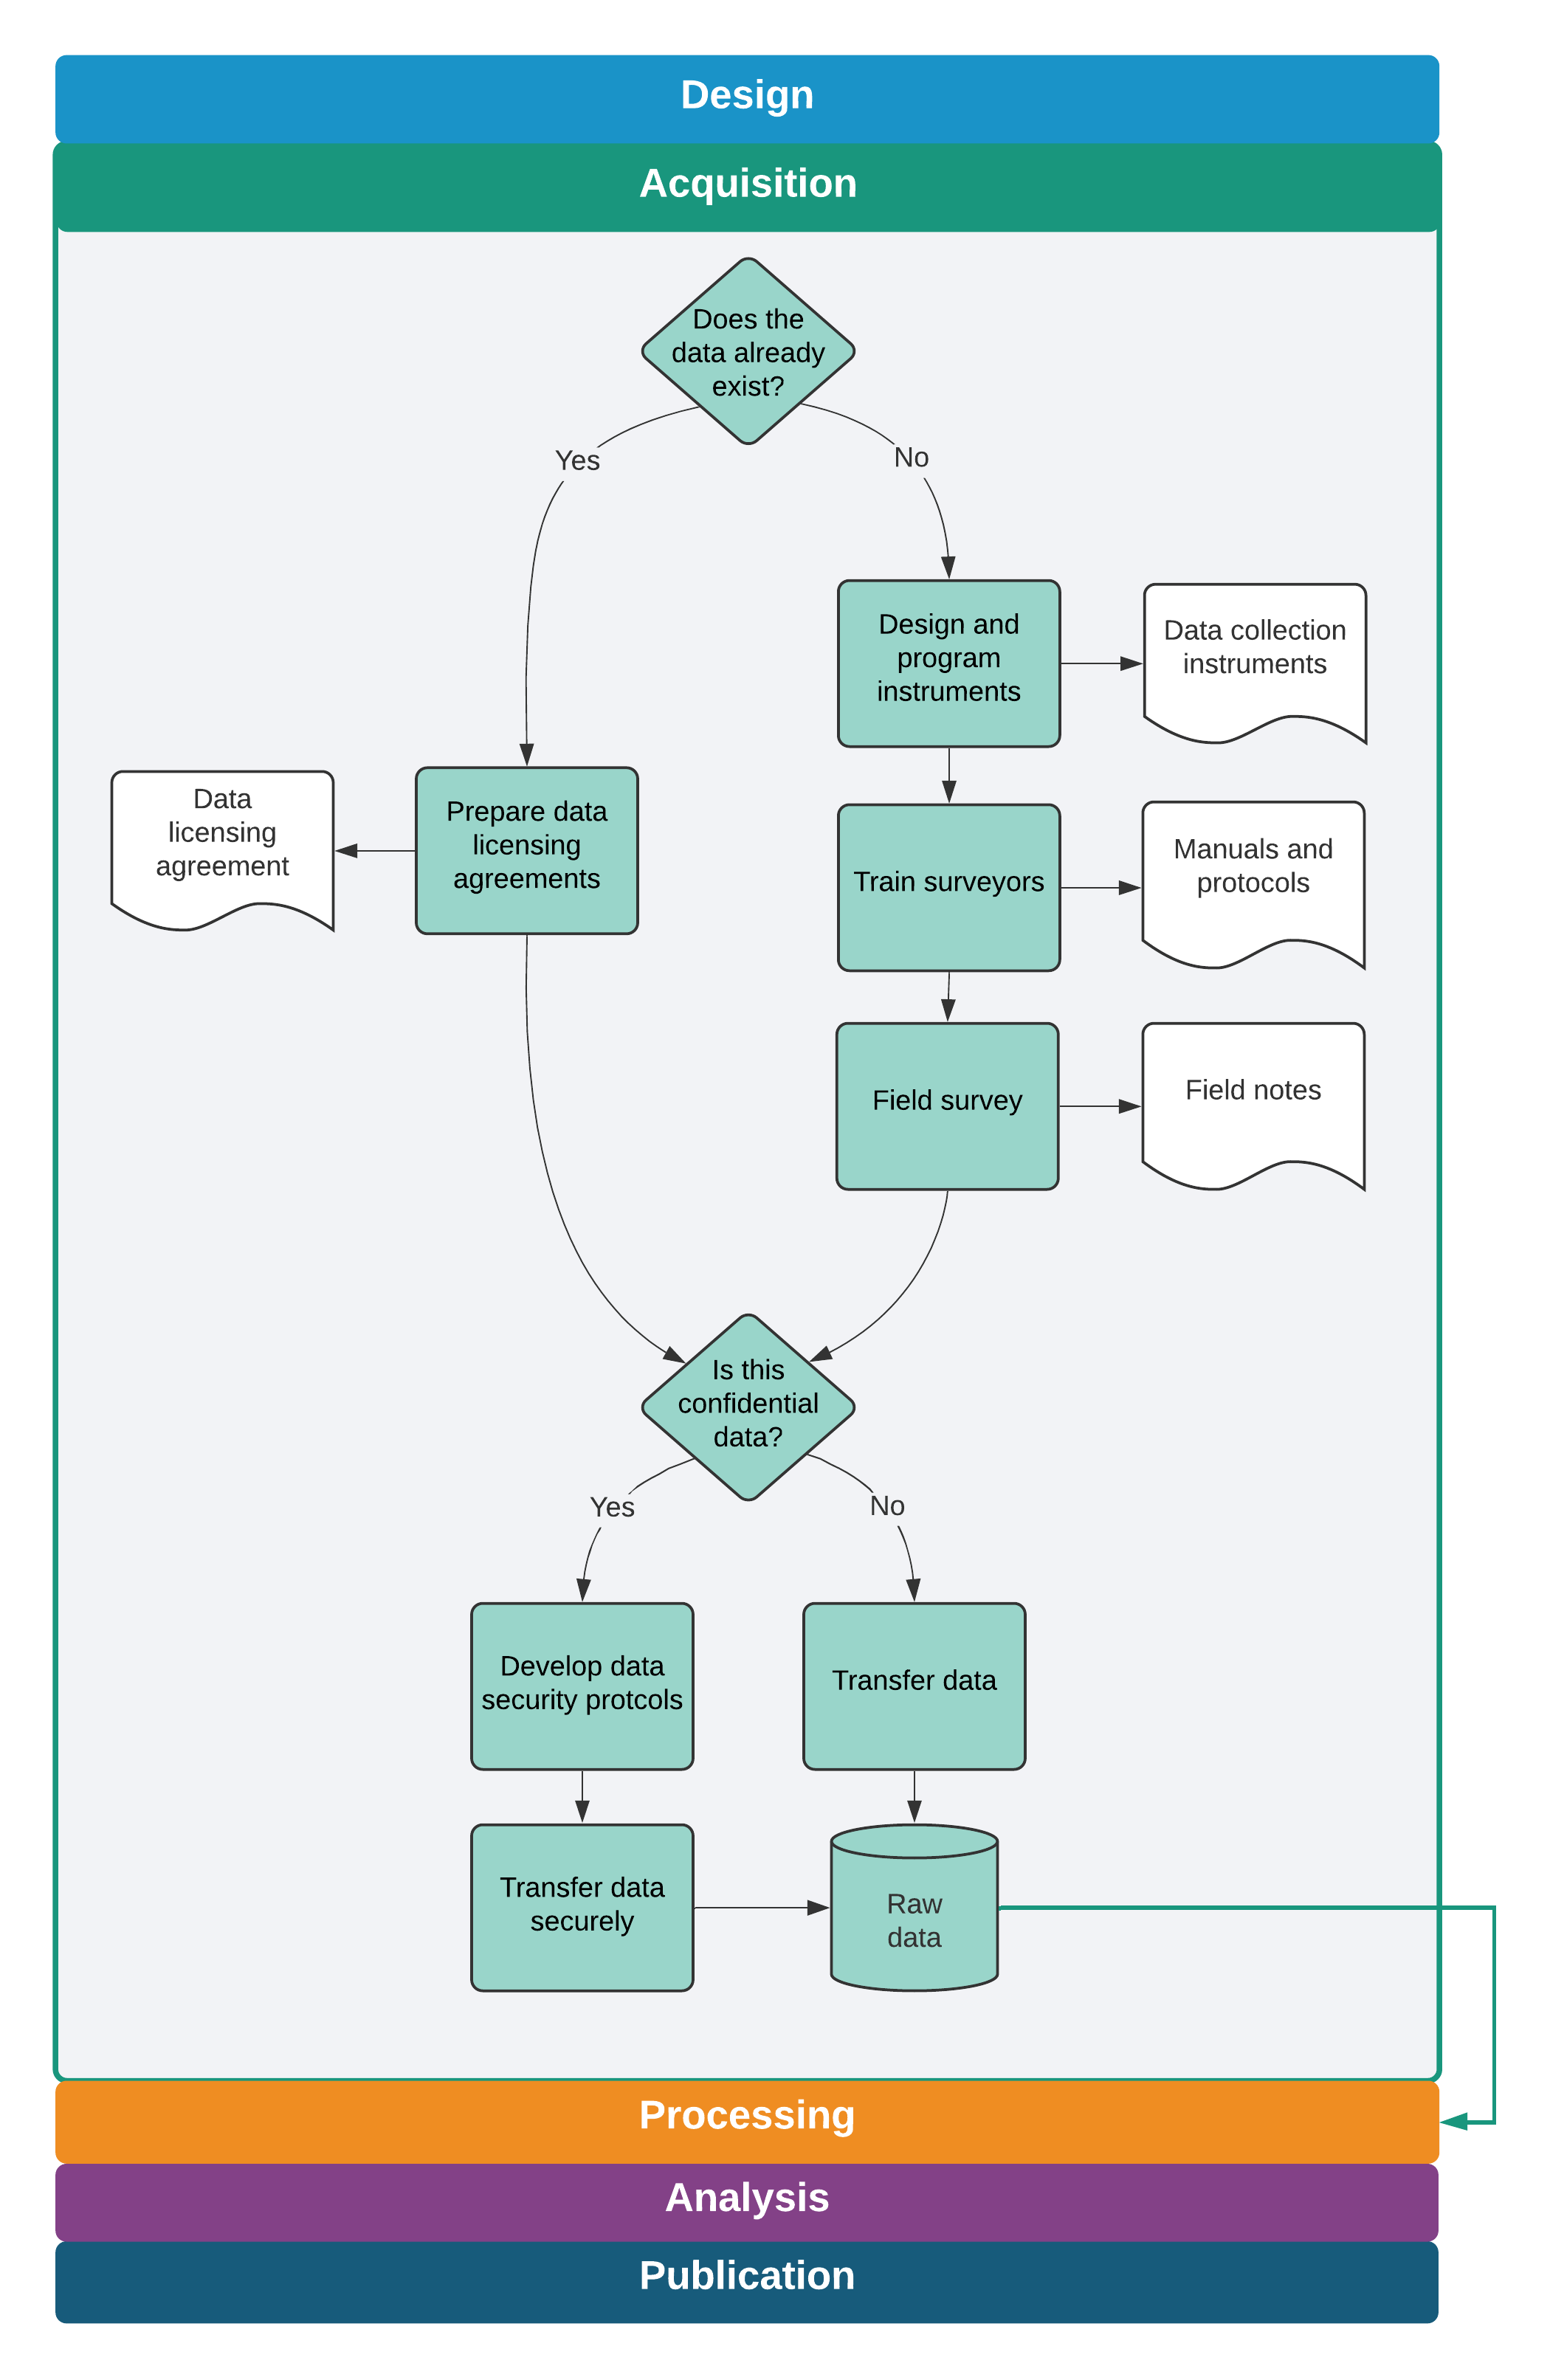
\includegraphics[width=1.5\linewidth]{diagrams/Acquisition}
	\end{figure}
\end{fullwidth}
